\documentclass[prb,preprint]{revtex4-1} 
% The line above defines the type of LaTeX document.
% Note that AJP uses the same style as Phys. Rev. B (prb).

\usepackage{amsmath}  % needed for \tfrac, \bmatrix, etc.
\usepackage{amsfonts} % needed for bold Greek, Fraktur, and blackboard bold
\usepackage{graphicx} % needed for figures
\usepackage{tabularx}

\begin{document}

\title{Superconductivity}
% In a long title you can use \\ to force a line break at a certain location.

\author{Jiajun Shi}
\email{jshi15@amherst.edu} 
\affiliation{Department of Physics, Smith College, Northampton, MA 01063}
\author{He Claudia Yun}
\email{hyun@smith.edu}
\affiliation{Department of Physics, Smith College, Northampton, MA 01063}

% See the REVTeX documentation for more examples of author and affiliation lists.

\date{\today}

%____________abstract____________________________________________

\begin{abstract}

\end{abstract}

\maketitle 

%____________Introduction____________________________________________
\section{Introduction}

%____________Experiment____________________________________________
\section{Experiment}
Temperature and resistance are measured for two different materials: $YBa_{2}Cu_{3}O_{7}$ (YBCO) and $Bi_{2}Sr{2}Ca_{2}Cu_{3}O_{9}$ (BISCO). The experiments are done in two different ways for different materials.\\
\subsection{YBCO}
The setup of YBCO experiment is shown in the Fig. \ref{setup}. The device (Fig. \ref{sample}), including the YBCO sample, a thermocouple, a current probe and a voltage probe, is put in a plastic-foam cup and immersed in sands, which serve as insulator. The box variable resistor in Fig. \ref{setup} is only used for keeping the free wires at a fixed place. \\

\begin{figure}[h]
\centering
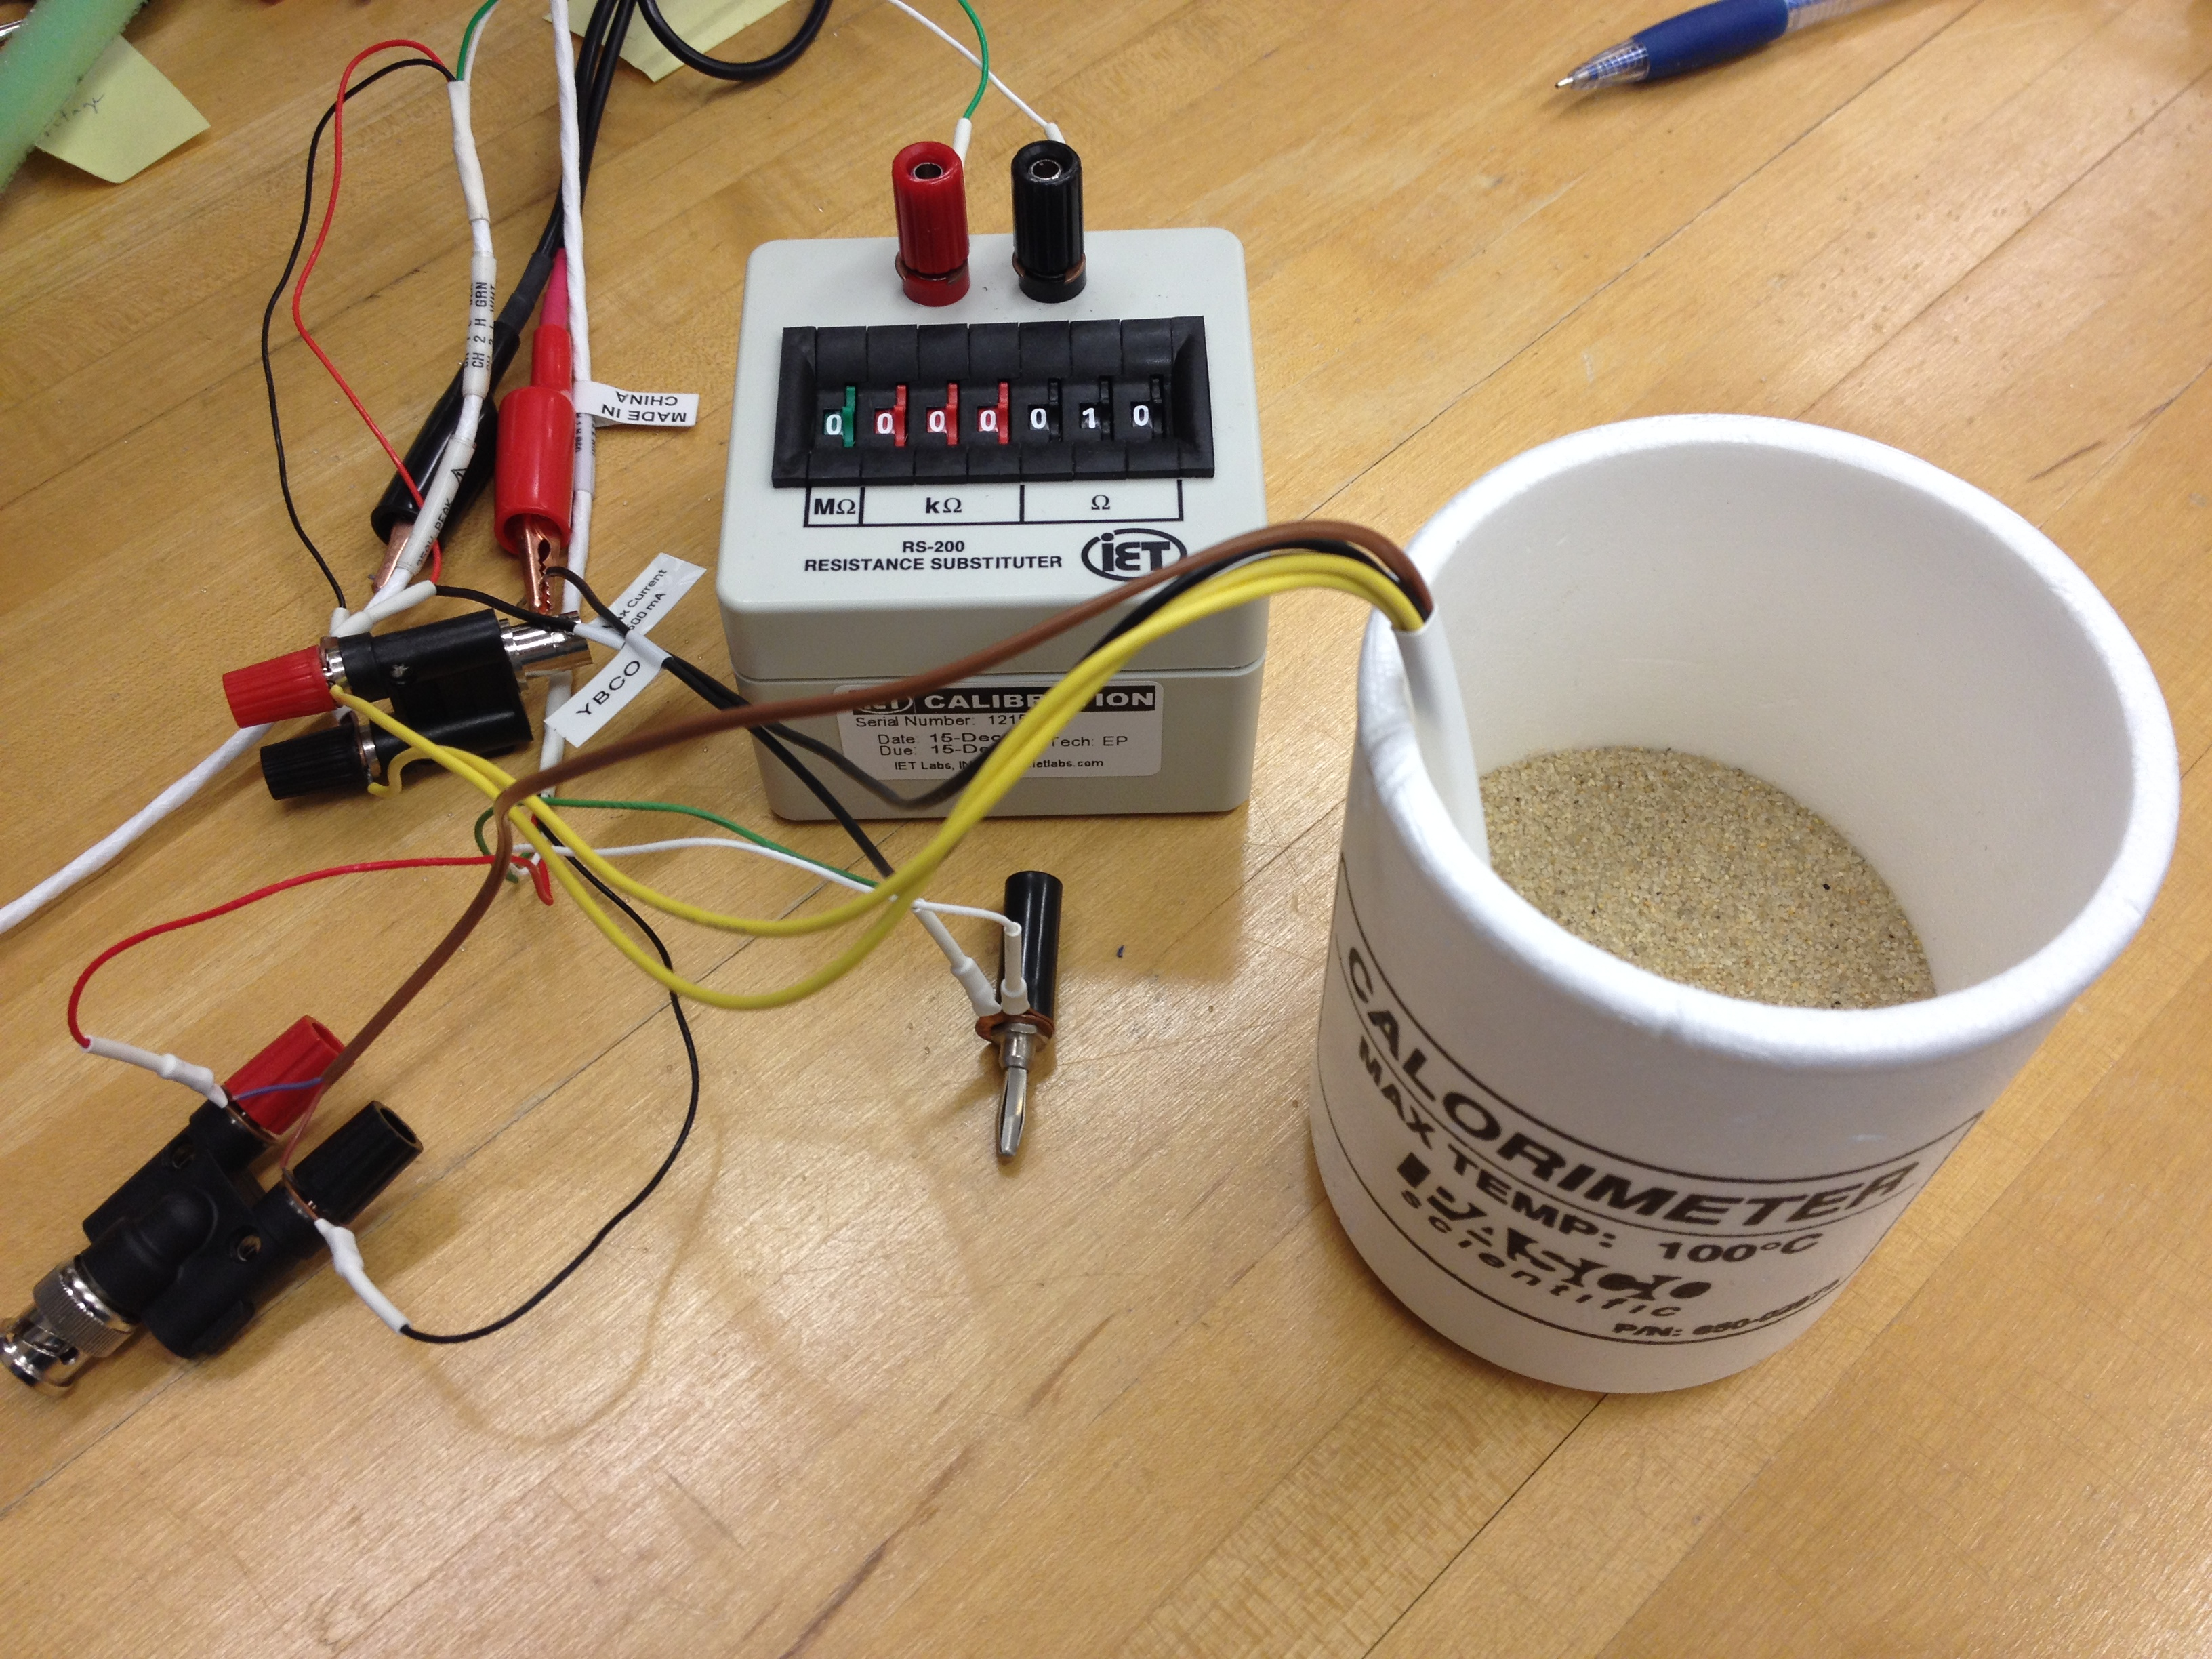
\includegraphics[width=14cm]{ybcosetup.jpg}
\caption{Picture of the experiment setup}
\label{setup}
\end{figure}

\begin{figure}[h]
\centering
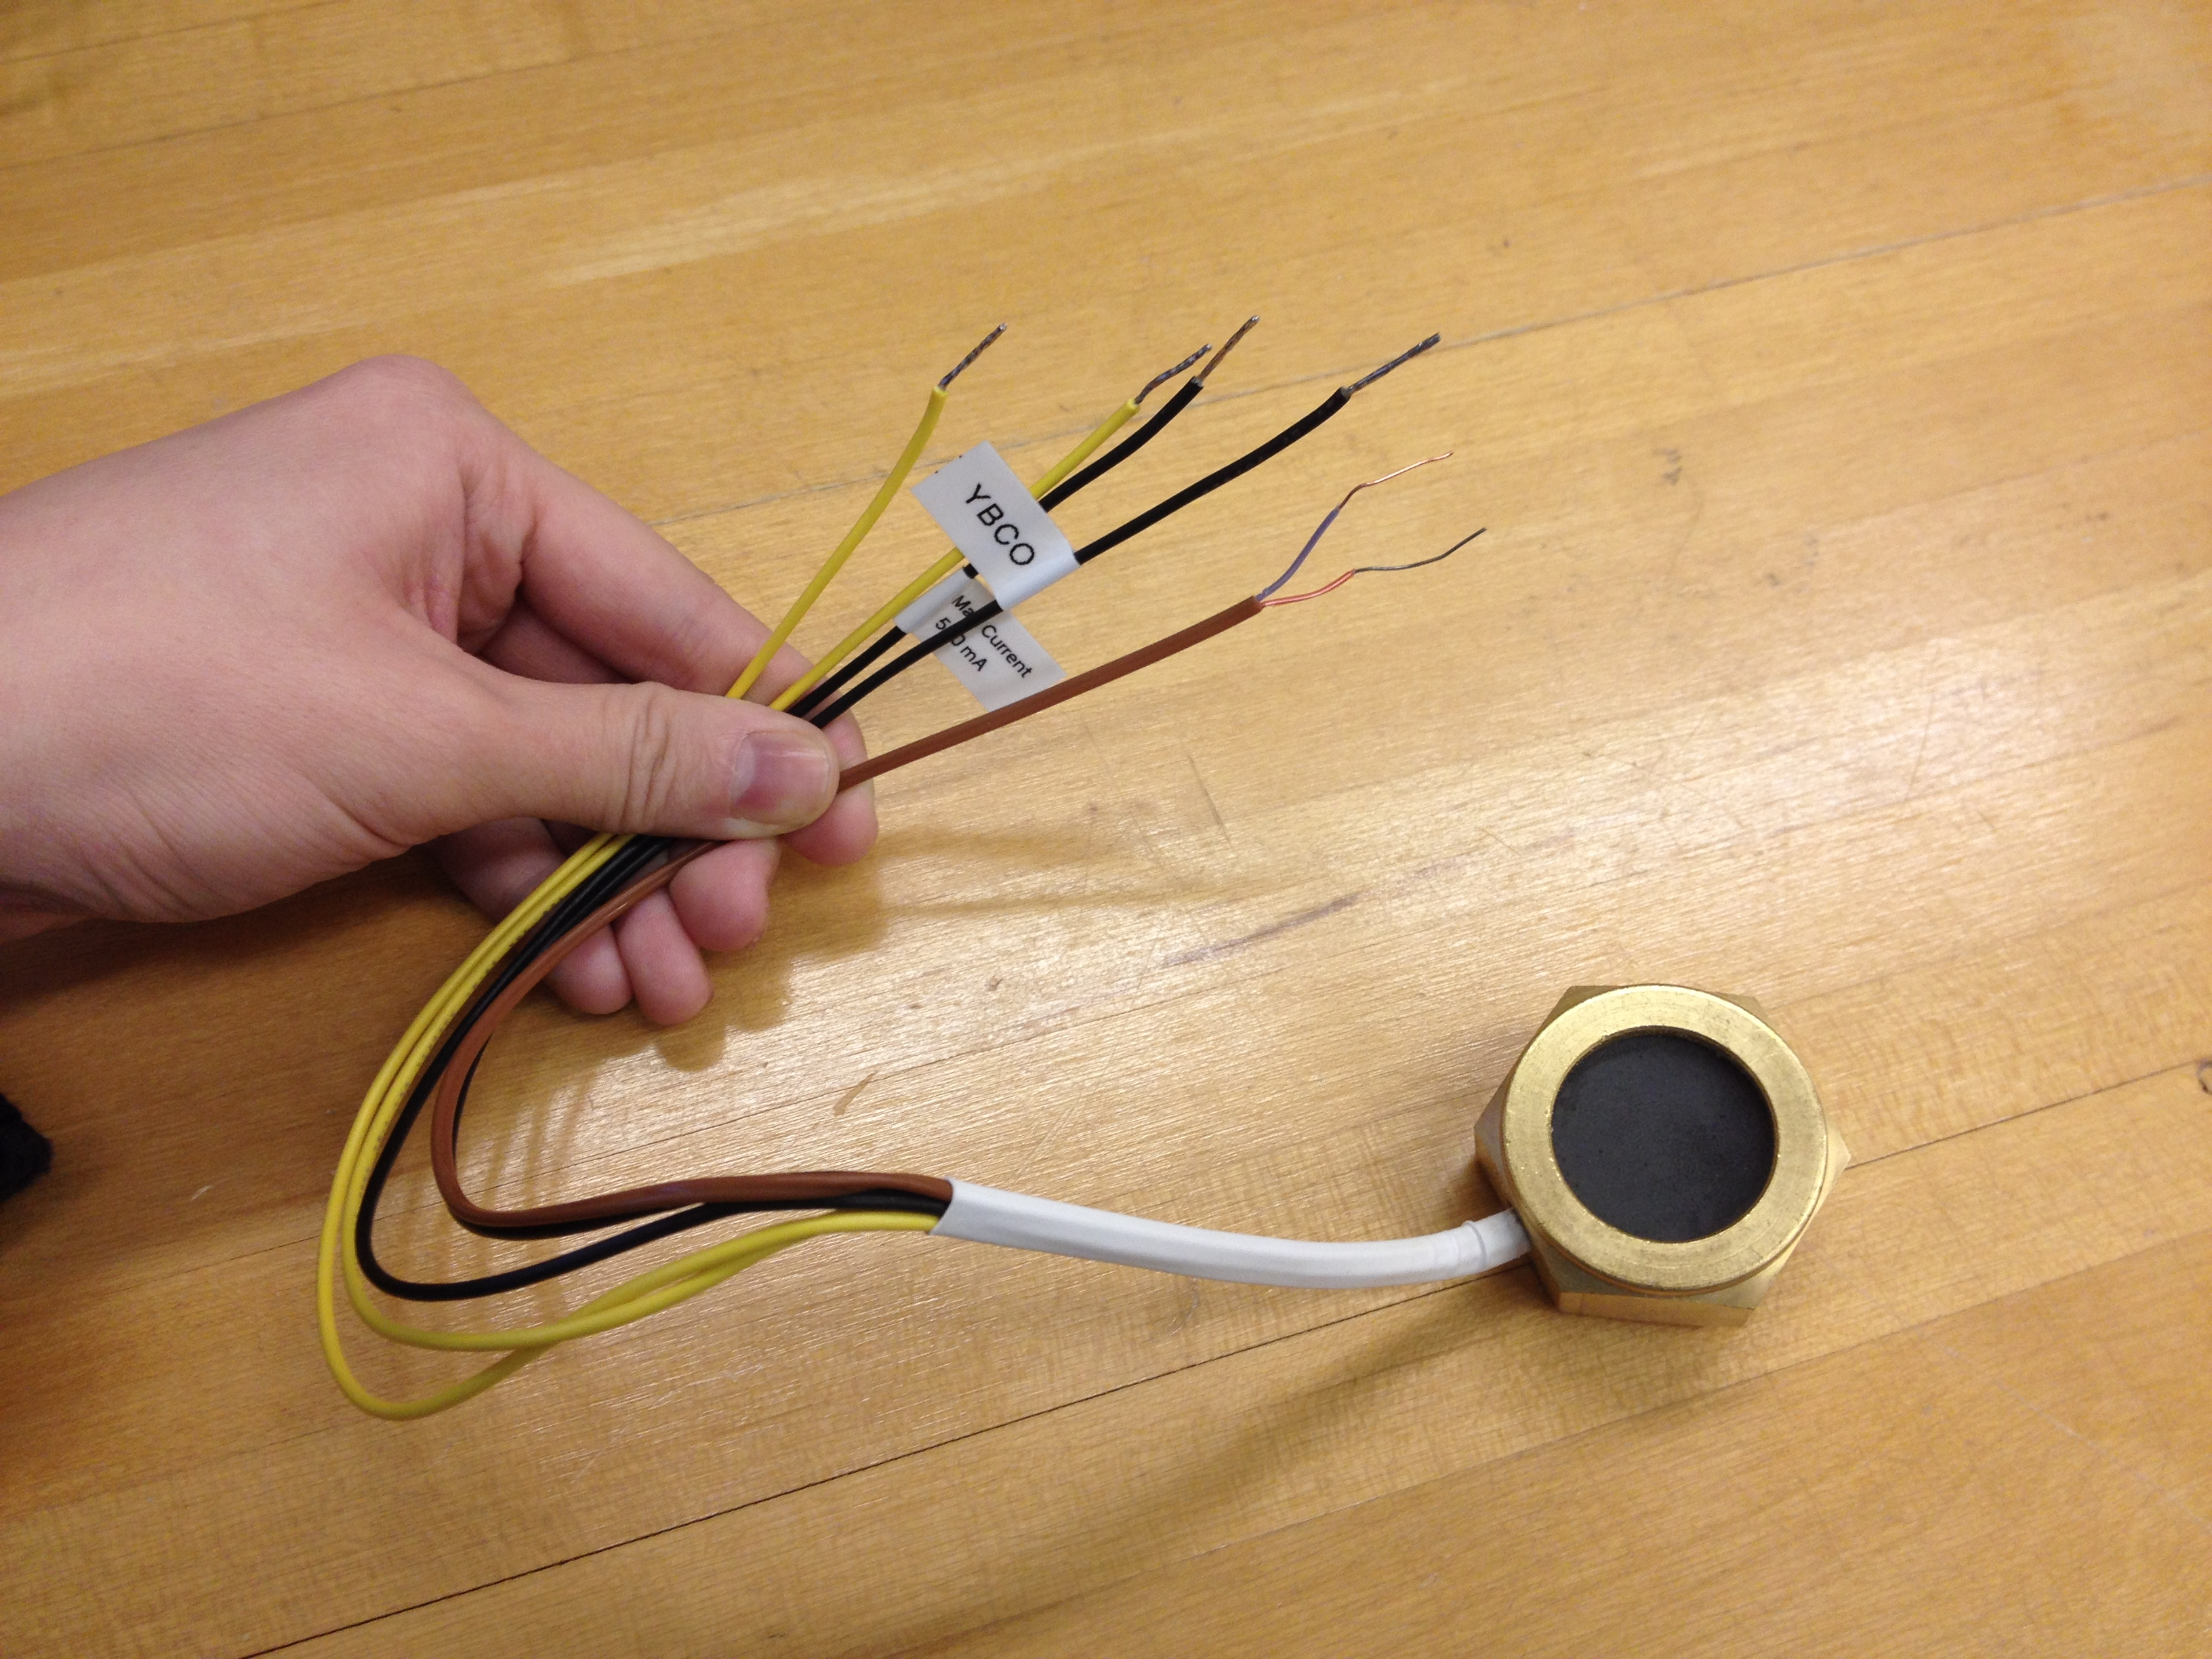
\includegraphics[width=14cm]{ybcosample.jpg}
\caption{Picture of the device, including YBCO sample (the black disk on top), thermocouple (brown lead), current (black leads) and voltage probes (yellow leads)}
\label{sample}
\end{figure}

When superconducting, the material has a very low resistance, which means the resistance of the leads of the probes becomes non-negligible. Therefore a method called four point probe is employed so that only the resistance of the material is measured, not that of the leads. The circuit is shown in Fig. \ref{fpp}. The black rectangle at the bottom represents the YBCO sample, an ammeter is connected in series with the sample through leads 1 and 4, and a voltmeter is connected in parallel with the sample through leads 2 and 3. Then the resistance of the sample could be calculated using Ohm's Law:

\begin{equation}
R=\frac{V}{I}
\label{ohm}
\end{equation}

where V and I are readings of the voltmeter and ammeter respectively. The key point here is that leads 2 and 3 have to be inside leads 1 and 4, in terms of position on the sample. Picture the meters as ideal meters plus lead resistance. The advantage of doing so is that the ammeter approximately measures the current through the sample, because the resistance of the voltmeter is so much bigger than that of the superconductor that the current through the voltmeter is very close to zero; and the voltmeter only measures the voltage across the sample. However, i f the position of the ammeter and voltmeter were switched, as shown in Fig. \ref{fpp2}, the voltmeter would measure the voltage across the lead resistance of the ammeter and the sample resistance connected in parallel. The total resistance of the two in parallel would differ from the sample resistance a lot because when superconducting, the resistance of the sample is comparable to the resistance of the lead. \\

\begin{figure}[h]
\centering
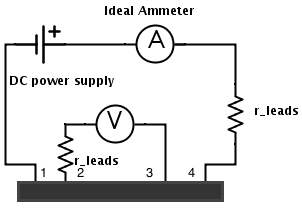
\includegraphics[width=8cm]{fourpointprobe2.png}
\caption{Schematic of four point probe}
\label{fpp}
\end{figure}

\begin{figure}[h]
\centering
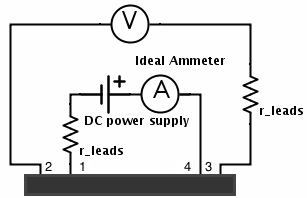
\includegraphics[width=8cm]{fourpointprobe3.png}
\caption{Schematic of the other (bad) configuration of four point probe}
\label{fpp2}
\end{figure}

The sample is connected to two digital multimeters (DMM) (top two in Fig. \ref{meters}) and one power source {bottom one in Fig. \ref{meters}}. The top one is measuring the voltage across the thermocouple, and the voltage can be translated into temperature according to the table in Fig. \ref{temp}. \\

\begin{figure}[h]
\centering
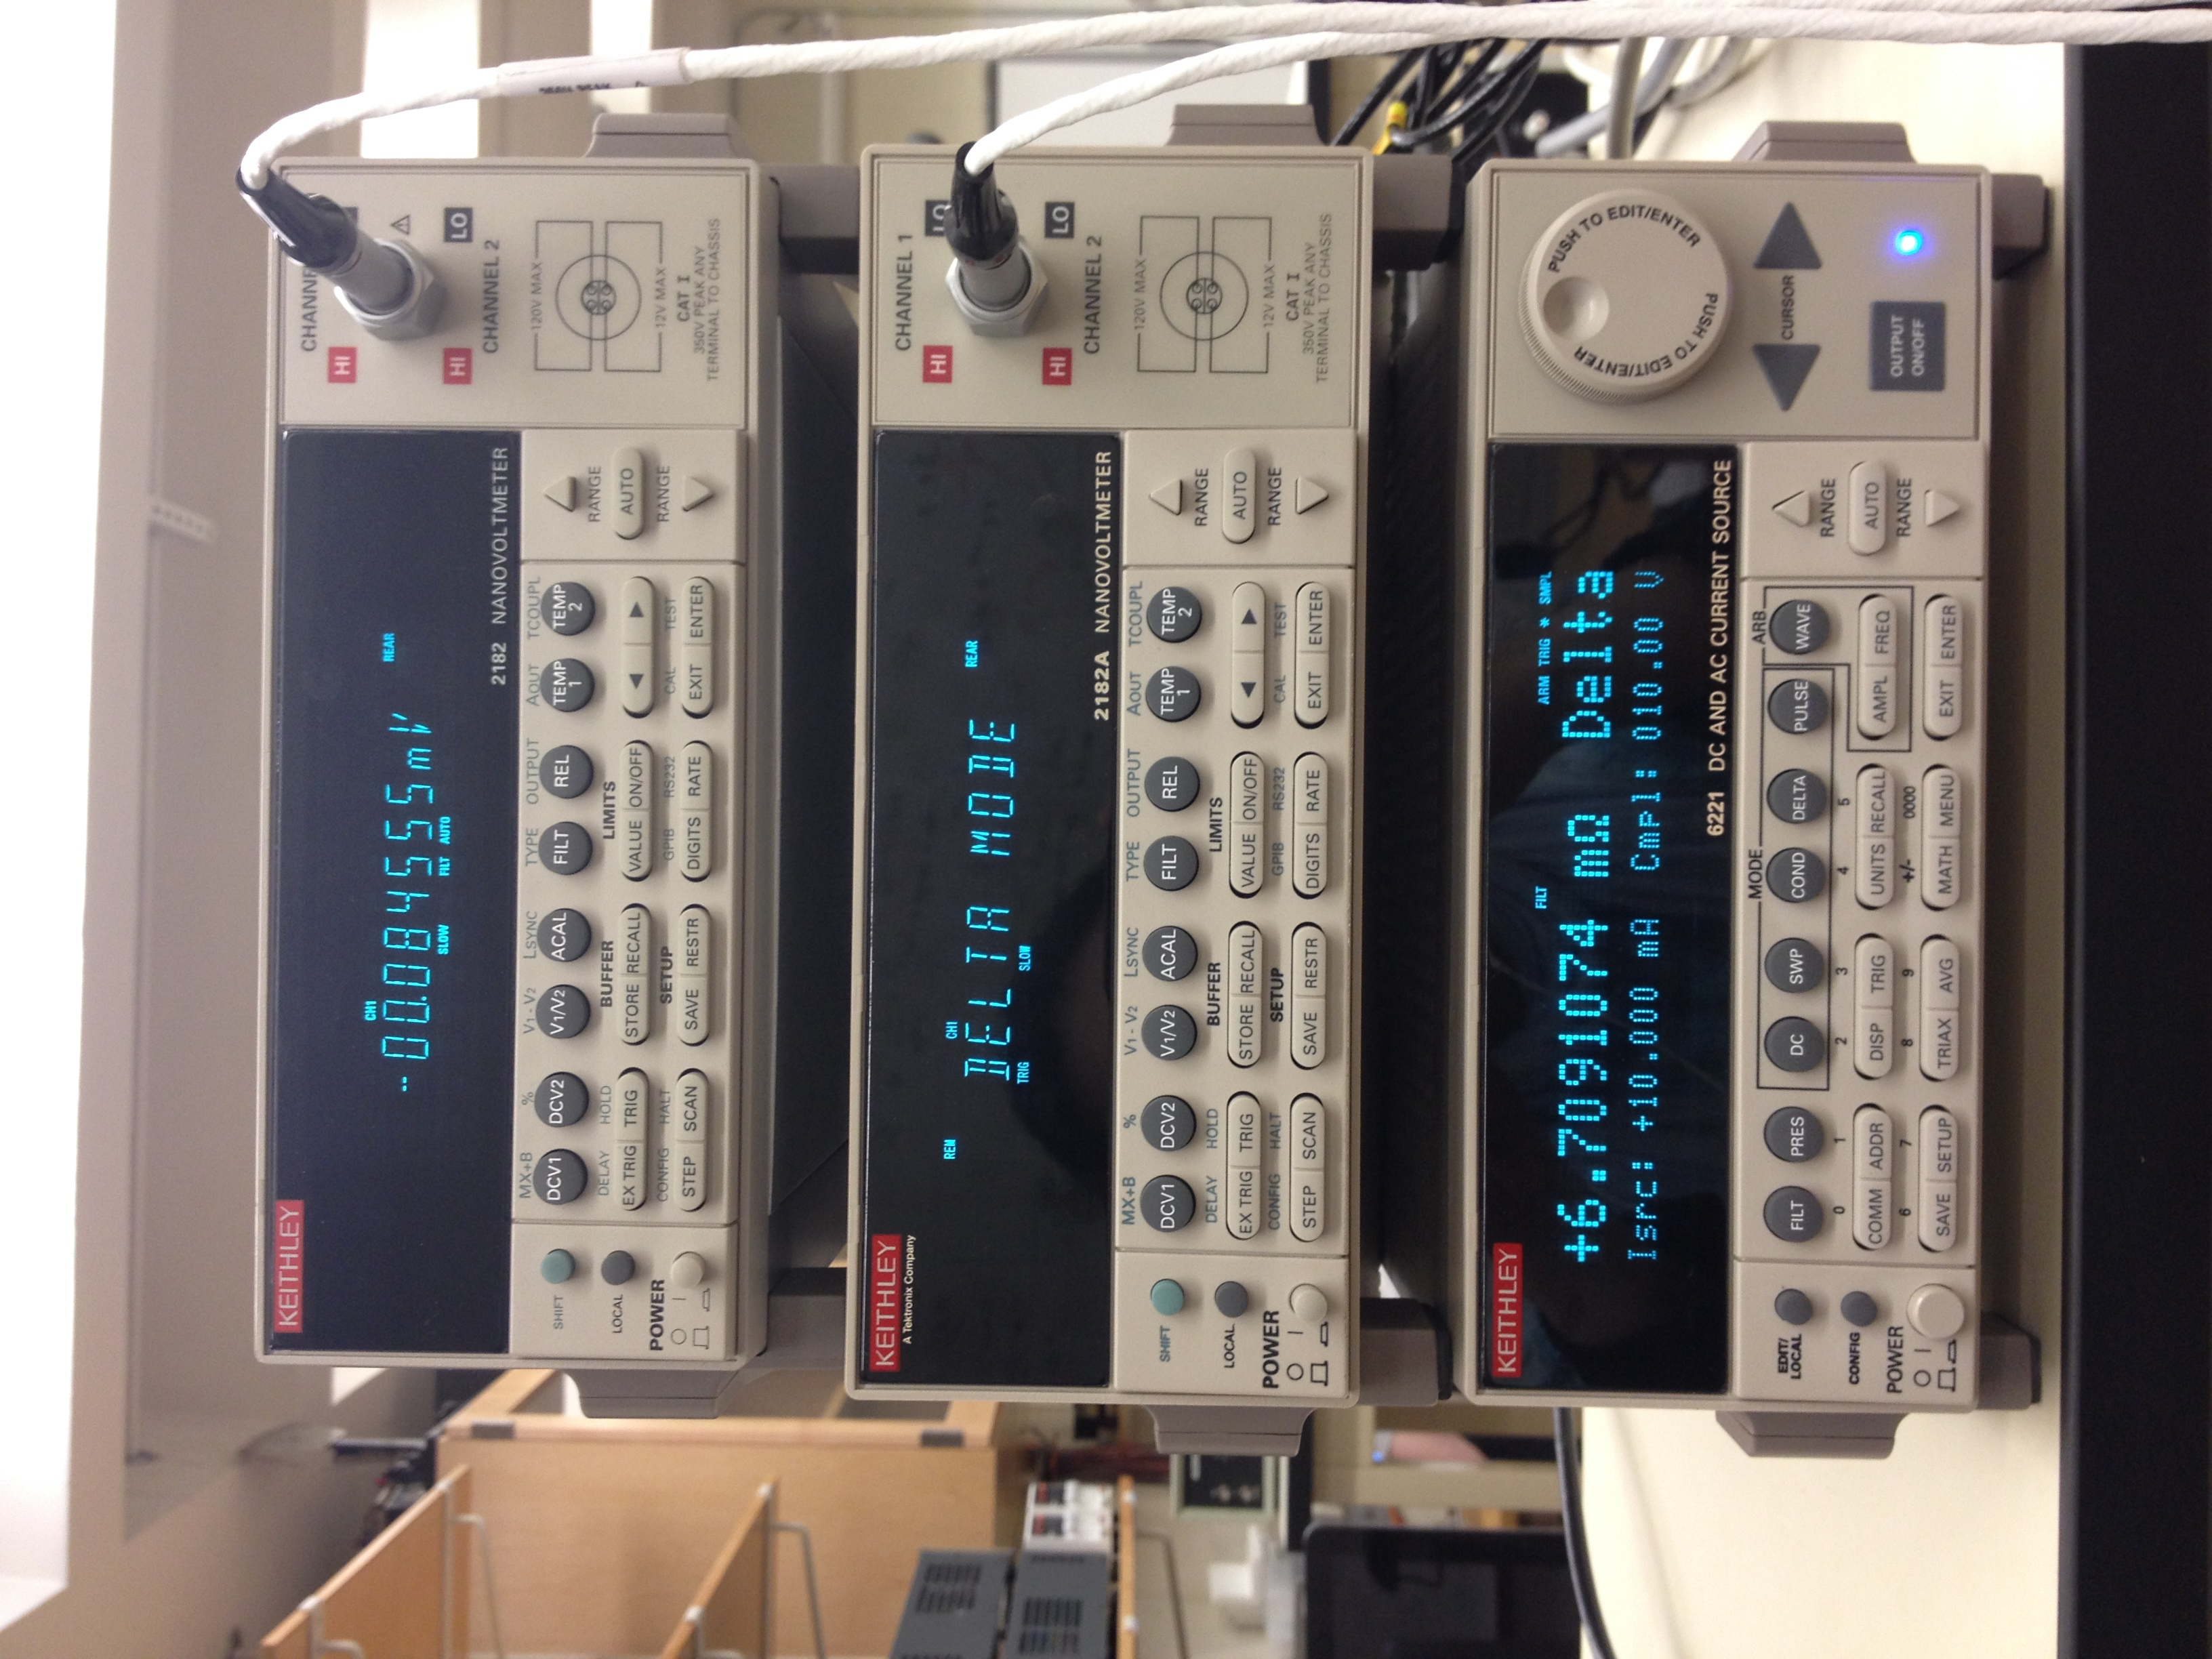
\includegraphics[width=10cm]{ybcometers.jpg}
\caption{The DMMs and power supply used. The top one measures the voltage of the thermocouple, the middle one measures the voltage across the sample, but the value is not shown on the screen under delta mode. And the bottom one is a power source that is in delta mode, and it reads the resistance of the YBCO sample.}
\label{meters}
\end{figure}

\begin{figure}[h]
\centering
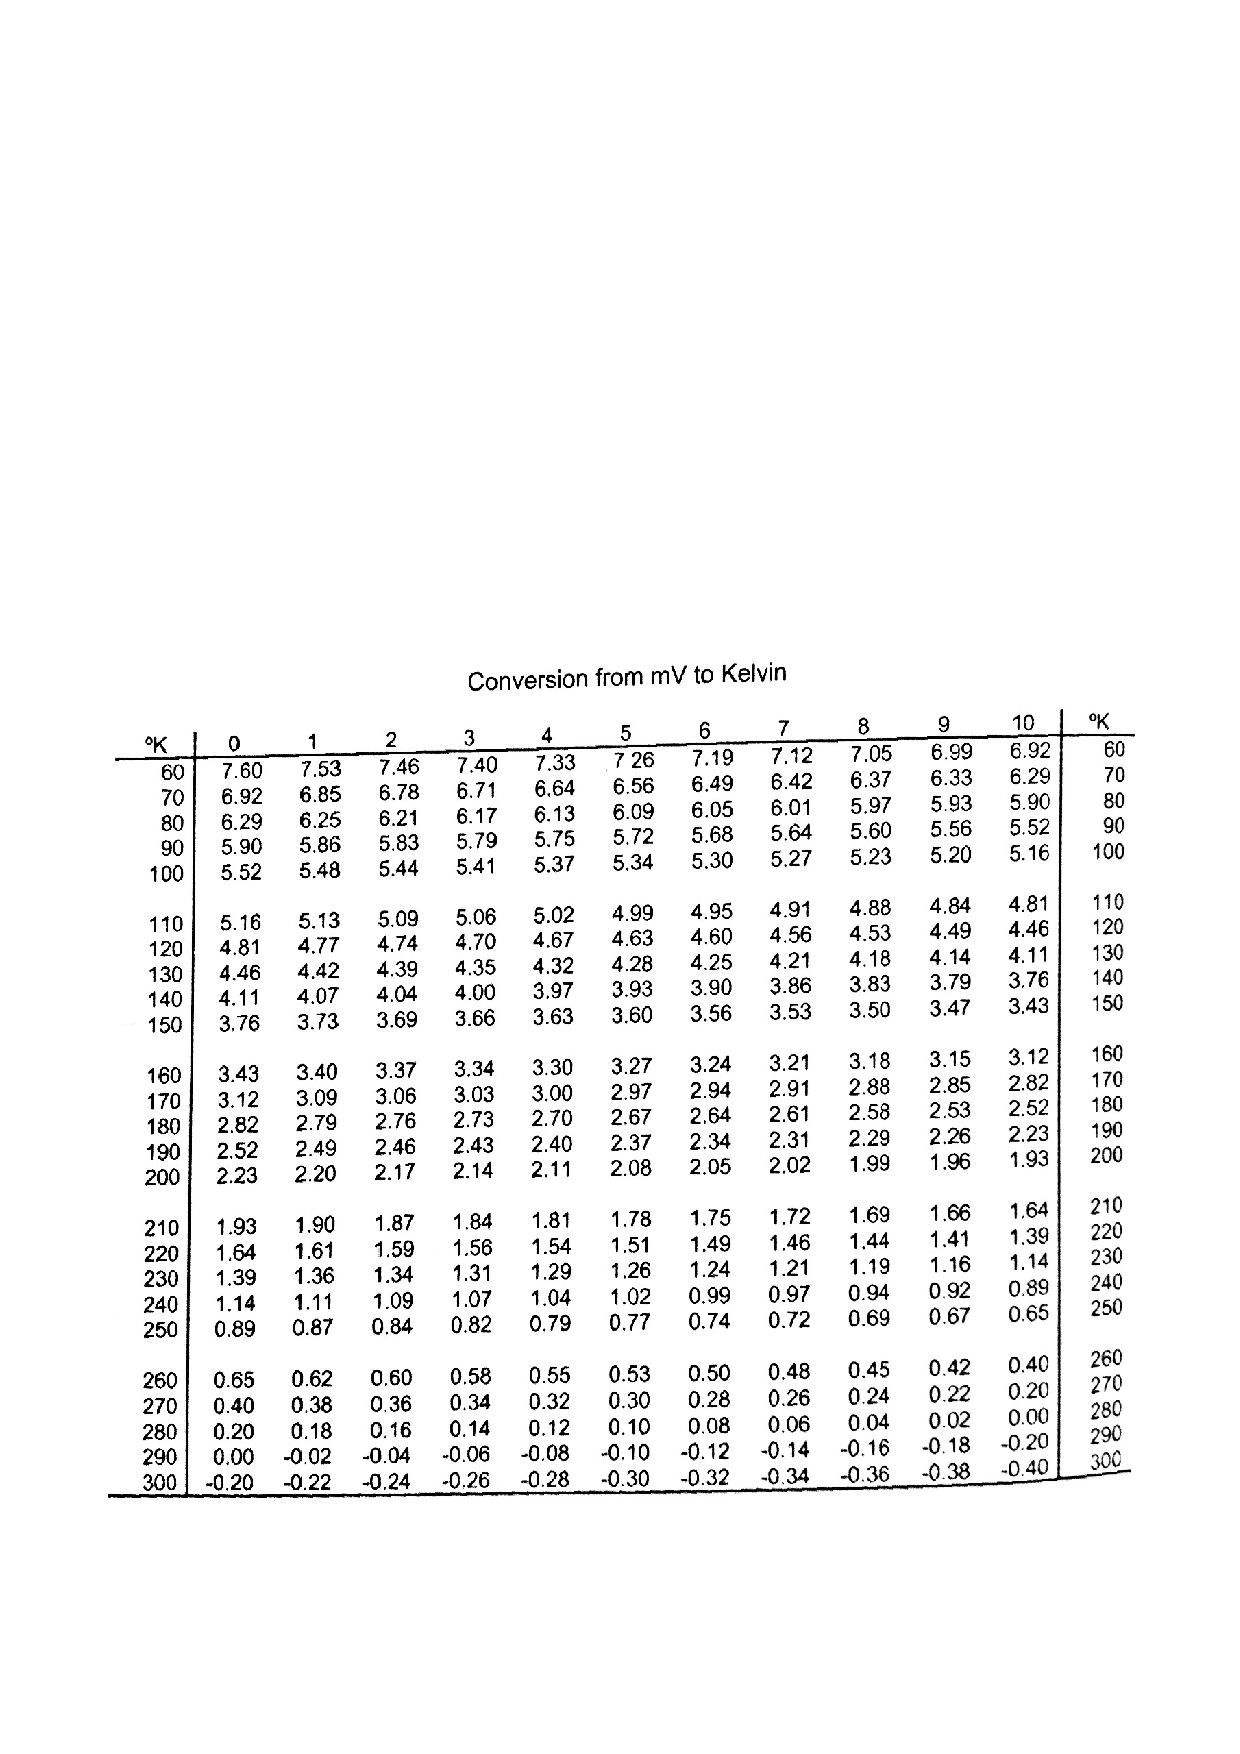
\includegraphics[width=14cm]{temperature.pdf}
\caption{The correlation between the temperature and the voltage across the thermocouple}
\label{temp}
\end{figure}

The source is the "DC power supply" in Fig. \ref{fpp} and Fig. \ref{fpp2}. Although it is labelled as DC power source, it is actually in delta mode, which means it is outputting a current alternating between positive and negative. The advantage of delta mode is that it can eliminate the affect of offsets measured by the voltmeter. When a positive current is passing through the sample, the voltmeter measures an offset and the real voltage signal across the sample, $V_{+}=V_{offset}+V_{signal}$; if the current is reversed, the voltage across the sample would also flip sign, but the offset would remain the same, $V_{-}=V_{offset}-V_{signal}$. From $V_{+}$ and $V_{-}$, the voltage due to the sample can be calculated. The middle DMM reads the two voltages and calculates $V_{signal}$ automatically. The middle DMM is also connected to the power supply at the back. The power source reads $V_{signal}$ from the middle DMM and then divides it by the current to get the resistance of the superconductor, which is shown on the screen in unit of m$\Omega$. By observing the temperature dependence of the resistance, the critical temperature of the superconductor could be found out. \\

However, the drawback of this setup is that we could not make computer record the data. So we videotaped the DMMs while the sample was cooled down by liquid nitrogen, and then transcribed the thermocouple voltage and superconductor resistance into analysis tool, i.e. Igor Pro, by hand. To test the current dependence of the critical temperature of the material, four sets of data are collected, with current output of the power supply being 0.1mA, 1mA, 10mA and 100mA respectively.\\

\subsection{BISCO}

The device of BISCO employs the same four point probe method. 


%____________Results____________________________________________
\section{Results}

\subsection{YBCO}

\subsection{BISCO}



%____________Discussion____________________________________________
\section{Discussion}

%____________Conclusion____________________________________________
\section{Conclusion}


\begin{acknowledgments}

We gratefully acknowledge Nathanael Fortune and Dana Parsons, who helped with the experimentation and editing of this experiment. This work was supported by the Smith College Physics Department.

\end{acknowledgments}


\begin{thebibliography}{99}

%\bibitem{wik} Double Slit Experiment, \url{<http://upload.wikimedia.org/wikipedia/commons/c/c2/Single_slit_and_double_slit2.jpg/>}.
\bibitem{drawcircuit} Scheme-it, \url{http://www.digikey.com/schemeit}
\bibitem{energy} Optical Pumping, \url{http://internal.physics.uwa.edu.au/~stamps/2006Y3Lab/SteveAndBlake/theoretical.html}

\end{thebibliography}

%\newpage   % Start a new page for tables

\end{document}
